\documentclass[12pt]{ctexart}

\newif\ifusebigeightk
\usebigeightkfalse

\ifusebigeightk
  \usepackage[paperwidth=390mm,paperheight=270mm,top=1.35cm,bottom=1.25cm,left=1.9cm,right=1.6cm]{geometry}
\else
  \usepackage[paperwidth=420mm,paperheight=297mm,top=1.5cm,bottom=1.4cm,left=2.0cm,right=1.8cm]{geometry}
\fi
\usepackage{amsmath,amssymb,mathtools}
\usepackage{array,tabularx,booktabs,multirow}
\usepackage{enumitem}
\usepackage{graphicx}
\usepackage{fancyhdr}
\usepackage{lastpage}
\usepackage{tikz}
\usepackage{setspace}
\usepackage[hidelinks]{hyperref}

\setlength{\parindent}{0pt}
\setlength{\parskip}{0.14em}
\setlength{\headheight}{15pt}
\setlist[enumerate]{itemsep=0.05em, topsep=0.05em}

\newcommand{\schoolname}{柏木体育}
\newcommand{\examyear}{2026}
\newcommand{\examtitle}{全国高等学校运动训练、武术与民族传统体育专业}
\newcommand{\papersubtitle}{单独统一招生考试 数学冲刺卷（四）}

\pagestyle{fancy}
\fancyhf{}
\fancyhead[L]{\schoolname}
\fancyhead[R]{数学试卷}
\fancyfoot[C]{\thepage}
\renewcommand{\headrulewidth}{0.4pt}
\renewcommand{\footrulewidth}{0pt}

\newcommand{\bindingline}{
  \begin{tikzpicture}[remember picture,overlay]
    \draw[densely dotted,line width=0.85pt]
      ([xshift=13.5mm,yshift=-18mm]current page.north west) --
      ([xshift=13.5mm,yshift=18mm]current page.south west);
    \node[rotate=90,anchor=south,font=\small]
      at ([xshift=18.5mm]current page.west) {装订线};
  \end{tikzpicture}
}
\AddToHook{shipout/background}{\bindingline}

\newcommand{\papertitleblock}{
  \begin{center}
    {\fontsize{18.5pt}{23pt}\selectfont\bfseries \schoolname\ \examyear\ 年全国高等学校运动训练、武术与民族\par}
    \vspace{0.08em}
    {\fontsize{18.5pt}{23pt}\selectfont\bfseries 传统体育专业\par}
    \vspace{0.5em}
    {\fontsize{19pt}{25pt}\selectfont\bfseries 单独统一招生考试\quad 数学冲刺卷（四）\par}
  \end{center}
}

\newcommand{\scoretable}{
  \renewcommand{\arraystretch}{1.45}
  \begin{center}
    \begin{tabularx}{0.86\textwidth}{|>{\centering\arraybackslash}m{1.55cm}|*{4}{>{\centering\arraybackslash}X|}}
      \hline
      题号 & 一 & 二 & 三 & 总分 \\
      \hline
      得分 &  &  &  &  \\
      \hline
    \end{tabularx}
  \end{center}
  \renewcommand{\arraystretch}{1}
}

\newcommand{\sectiontitle}[1]{
  \vspace{0.18em}
  {\large\bfseries #1\par}
  \vspace{0.04em}
}

\newcommand{\blankline}[1][6cm]{\underline{\makebox[#1][s]{\hfill}}}

\newenvironment{choicequestions}{
  \begin{enumerate}[label=\arabic*., leftmargin=1.8em, itemsep=0.12em, topsep=0.08em]
}{
  \end{enumerate}
}

\newcommand{\choiceoptions}[4]{
  \par\noindent\vspace{0.02em}
  \begin{tabular*}{0.95\textwidth}{@{\extracolsep{\fill}}>{\raggedright\arraybackslash}p{0.21\textwidth}>{\raggedright\arraybackslash}p{0.21\textwidth}>{\raggedright\arraybackslash}p{0.21\textwidth}>{\raggedright\arraybackslash}p{0.21\textwidth}}
    A.\ #1 & B.\ #2 & C.\ #3 & D.\ #4
  \end{tabular*}
  \par\vspace{0.16em}
}

\newcommand{\choiceoptionslong}[4]{
  \par\noindent\vspace{0.02em}
  \begin{tabular*}{0.95\textwidth}{@{\extracolsep{\fill}}>{\raggedright\arraybackslash}p{0.445\textwidth}>{\raggedright\arraybackslash}p{0.445\textwidth}}
    A.\ #1 & B.\ #2 \\[0.32em]
    C.\ #3 & D.\ #4
  \end{tabular*}
  \par\vspace{0.16em}
}

\newenvironment{fillquestions}{
  \begin{enumerate}[label=\arabic*., leftmargin=1.8em]
}{
  \end{enumerate}
}

\newenvironment{solutionquestions}{
  \begin{enumerate}[label=\arabic*., leftmargin=1.8em]
}{
  \end{enumerate}
}

\newcommand{\spreadpair}[2]{%
  \noindent
  \begin{minipage}[t][0.945\textheight][t]{0.486\textwidth}
    #1
  \end{minipage}\hfill
  \begin{minipage}[t][0.945\textheight][t]{0.486\textwidth}
    #2
  \end{minipage}%
}

\begin{document}

\spreadpair{
  \papertitleblock
  \scoretable

  \sectiontitle{一、选择题：本大题共 8 小题，每小题 8 分，共 64 分。}

  \begin{choicequestions}
  \item 已知集合 $A=\{0,1,2,3\}$，$B=\{x \in \mathbb{Z}\mid 2x-5<0\}$，则集合 $A\cap B$ 的元素个数为（\quad）
  \choiceoptions{3}{4}{5}{6}

  \item 下列函数中，在区间 $(-\infty,0)$ 上单调递减的是（\quad）
  \choiceoptions{$f(x)=xe^x$}{$f(x)=\sin 2x$}{$f(x)=x^2+2x$}{$f(x)=|x|$}

  \item 在等差数列 $\{a_n\}$ 中，$a_4+a_5+a_6=15$，则 $a_2+a_8=(\quad)$
  \choiceoptions{10}{7}{6}{5}

  \item 现将 5 名志愿者分配到 4 个服务点，要求每位志愿者都要到一个服务点服务，每个服务点都要安排志愿者，有（\quad）种分配方式
  \choiceoptions{36}{60}{240}{1440}

  \item 设 $a=3^{-0.2}$，$b=3^{0.2}$，$c=\log_3 0.2$，则 $a,b,c$ 的大小关系为（\quad）
  \choiceoptions{$c<b<a$}{$c<a<b$}{$a<b<c$}{$a<c<b$}

  \item 若双曲线 $\dfrac{x^2}{a^2}-\dfrac{y^2}{b^2}=1\,(a>0,b>0)$ 的一条渐近线方程为 $y=2x$，则该双曲线的离心率为（\quad）
  \choiceoptions{$\dfrac{1}{2}$}{$\dfrac{\sqrt{5}}{5}$}{2}{$\sqrt{5}$}

  \item 已知函数 $f(x)=\sin\!\left(x+\dfrac{\pi}{3}\right)\cos x$，则（\quad）
  \choiceoptionslong{$f(x)=\dfrac{1}{2}\sin\!\left(2x+\dfrac{\pi}{6}\right)$}{$f(x)$ 的最大值为 $2$}{$y=f(x)$ 的图象关于直线 $x=-\dfrac{\pi}{12}$ 对称}{$f(x)$ 在区间 $\left(0,\dfrac{\pi}{12}\right)$ 上单调递增}

  \item 设 $\alpha,\beta$ 是两个平面，$m,l$ 是两条直线，则下列命题为真命题的是（\quad）
  \choiceoptionslong{若 $\alpha \perp \beta$，$m\parallel \alpha$，$l\parallel \beta$，则 $m\perp l$}{若 $m\subset \alpha$，$l\subset \beta$，$m\parallel l$，则 $\alpha\parallel \beta$}{若 $\alpha\cap \beta=m$，$l\parallel \alpha$，$l\parallel \beta$，则 $m\parallel l$}{若 $m\perp \alpha$，$l\perp \beta$，$m\parallel l$，则 $\alpha\perp \beta$}
  \end{choicequestions}
}{
  \sectiontitle{二、填空题：本大题共 4 小题，每小题 8 分，共 32 分。}

  \begin{fillquestions}
  \setcounter{enumi}{8}
  \item 若某射手每次射击击中目标的概率均为 $\frac{2}{3}$，每次射击的结果相互独立，则在他连续 4 次射击中，恰好有两次击中目标的概率为 \blankline[5.8cm]。
  \item 已知数列 $\{a_n\}$ 的前 $n$ 项和 $s_n=n^2+n$，则 $a_n=$ \blankline[4.7cm]。
  \item 在 $\triangle ABC$ 中，$AC=7$，$BC=4$，点 $D$ 满足 $\overrightarrow{AD}=2\overrightarrow{DB}$，$CD=\sqrt{19}$，则 $BD=$ \blankline[5.2cm]。
  \item 已知三棱锥 $P-ABC$ 中，$AB=BC=AC=3$，$PA=6$，当 $PA\perp$ 平面 $ABC$ 时，其外接球的表面积为 \blankline[5.6cm]。
  \end{fillquestions}

  \sectiontitle{三、解答题：本大题共 3 小题，每题 18 分，共 54 分。}

  \begin{solutionquestions}
  \setcounter{enumi}{12}
  \item 已知函数 $f(x)=xe^x-1$。
  \begin{enumerate}[label=(\arabic*), leftmargin=2em]
    \item 求 $f(x)$ 在点 $(0,f(0))$ 处的切线方程；
    \item 求 $f(x)$ 的极值。
  \end{enumerate}
  \end{solutionquestions}
}

\clearpage

\spreadpair{
  \vspace*{0.4em}
  \textbf{14.} 已知椭圆
  $E:\dfrac{x^2}{a^2}+\dfrac{y^2}{b^2}=1\,(a>b>0)$
  的左、右顶点分别为 $A,B$，且 $|AB|=4\sqrt{2}$，椭圆 $E$ 的焦距为 $4$。

  \vspace{1em}
  \begin{enumerate}[label=(\arabic*), leftmargin=2em, itemsep=0.9em]
    \item 求椭圆 $E$ 的标准方程；
    \item 已知点 $M$（$M$ 不在 $x$ 轴上）在椭圆 $E$ 上，直线 $AM$ 交 $y$ 轴于点 $P$，直线 $BM$ 交 $y$ 轴于点 $Q$，求 $|OP|\cdot|OQ|$ 的值。
  \end{enumerate}
}{
  \vspace*{0.4em}
  \textbf{15.} 如图，直四棱柱
  $ABCD-A_1B_1C_1D_1$
  的底面是边长为 $2$ 的菱形，$\angle ABC=60^\circ$，$AA_1=\sqrt{6}$。

  \vspace{1em}
  \begin{enumerate}[label=(\arabic*), leftmargin=2em, itemsep=0.9em]
    \item 求证：$A_1C_1\perp \text{平面}\,BDD_1$；
    \item 求直线 $AC_1$ 与平面 $ABB_1A_1$ 所成角的正切值。
  \end{enumerate}

  \vspace{0.3em}
  \begin{flushright}
    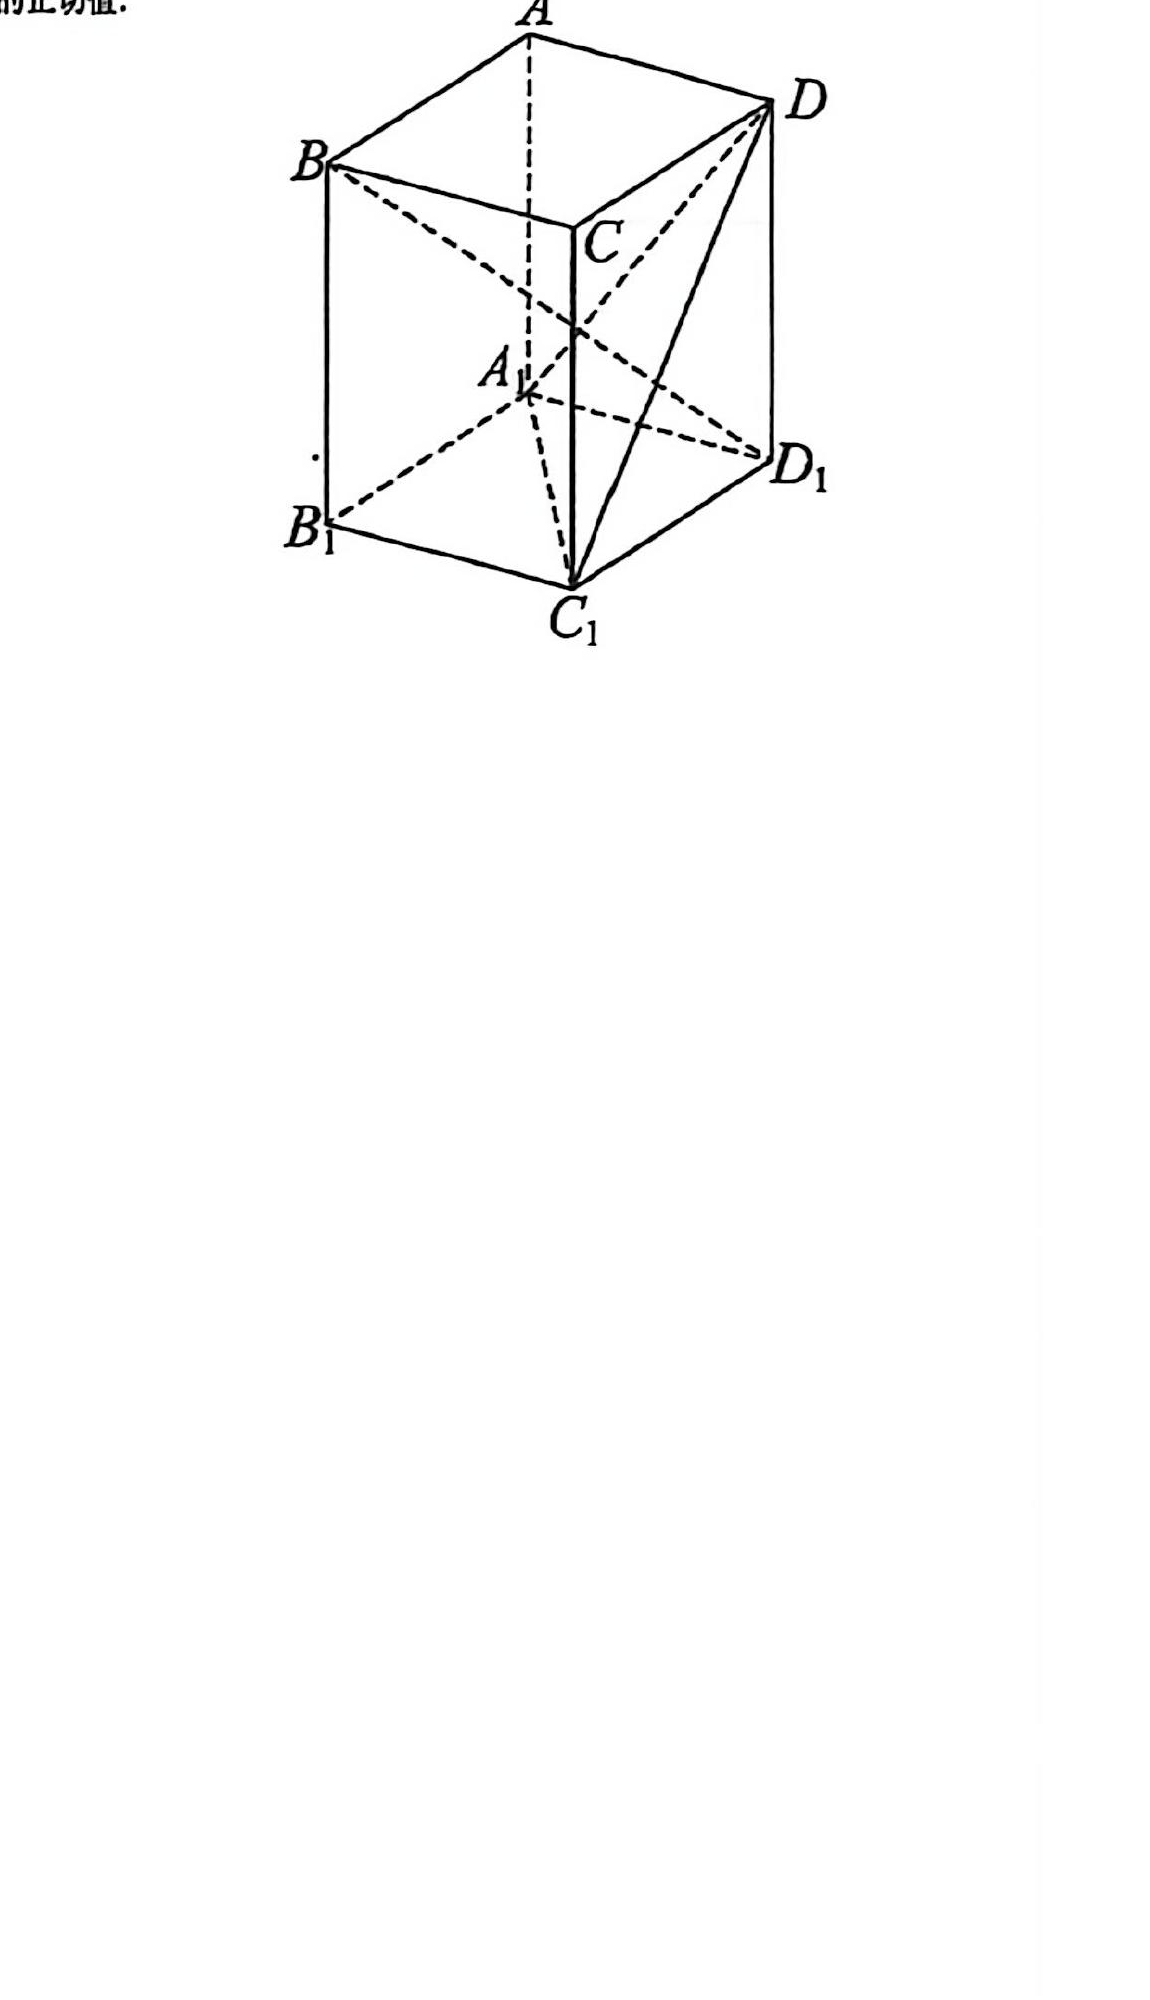
\includegraphics[width=0.58\textwidth]{q15-figure.png}
  \end{flushright}
}

\end{document}
